\documentclass[main.tex]{subfiles} % Subfile-Class

%==============================================================================%
%                                   Subfile                                    %
%==============================================================================%

\begin{document}

% Template

\section{Aufgabenstellung}

Die Aufgabenstellung des Moduls Produktentwicklung (PREN) 2 der
Hochschule Luzern fordert das interdisziplinäre Team heraus, ein autonomes 
Fahrzeug zu entwickeln. Das Fahrzeug muss sich durch ein vorgegebenes Wegenetzwerk autonom navigieren können, welches in der Abbildung~\ref{fig:Wegenetzwerk_Aufgabenstellung} dargestellt ist.
Dabei muss das autonome Fahrzeug im Wegenetzwerk Hindernisse bewältigen, gesperrte Wegpunkte meiden und eine optimale 
Route zum Ziel unter Berücksichtigung unbekannter Einschränkungen finden.

Das Team, das sich aus Studierenden der Fachrichtung Elektrotechnik, Informatik und Maschinenbau 
zusammensetzt, vereint ein breites Spektrum an technischen Kompetenzen. Im Rahmen der Projektphase von PREN 1 
erfolgte die Entwicklung eines Gesamtkonzepts, das nun in PREN 2 schrittweise in die Praxis umgesetzt wird.

Zu den wichtigsten Anforderungen zählen:
\begin{itemize}
    \item \textbf{Erkennung gesperrter Wegpunkte:} Pylonen müssen selbstständig detektiert werden.
    \item \textbf{Bewältigung von Hindernissen:} Hindernisse sollen aktiv entfernt und zurückgestellt werden.
    \item \textbf{Anpassung an veränderte Bedingungen:} Fehlende Streckenabschnitte müssen als nicht passierbar erkannt werden.
    \item \textbf{Autonome Zielfindung:} Über eine Zielauswahl vor dem Start soll das Fahrzeug die effizienteste Route zu einem vorgegebenen Ziel finden.
\end{itemize}

Zudem werden bei der Umsetzung strenge Vorgaben zu Dimensionen, Gewicht und
Autonomie des Systems berücksichtigt.

Die wissenschaftliche Herausforderung besteht darin, Sensorik, Elektronik 
und Algorithmen so zu kombinieren, dass eine zuverlässige Wegfindung und 
Hindernisbewältigung gewährleistet ist. Dabei liegt ein besonderes Augenmerk auf 
eine methodische Herangehensweise, die auch Nachhaltigkeitsaspekte berücksichtigt.

Das Projekt bietet die Möglichkeit, theoretisches Wissen praktisch 
anzuwenden und die Kompetenzen in interdisziplinärer Zusammenarbeit 
und systematischer Produktentwicklung zu vertiefen.

\begin{figure}[H]
    \centering
    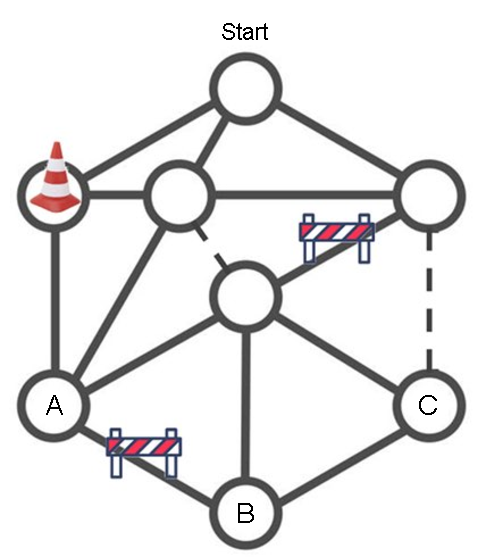
\includegraphics[width=0.25\textwidth]{Wegenetzwerk_Aufgabenstellung.pdf}
    \caption{Beispiel eines Wegenetzwerkes}~\label{fig:Wegenetzwerk_Aufgabenstellung}
\end{figure}


\end{document}